%%%%%%%%%%%%%%%%%%%%%%%%%%%%%%%%%%%%%%%%%%%%%%%%%%%%%%%%%%%%%%%%%%%%%%%%%%%%%
%%%                                FOLDER                                 %%%
%%%%%%%%%%%%%%%%%%%%%%%%%%%%%%%%%%%%%%%%%%%%%%%%%%%%%%%%%%%%%%%%%%%%%%%%%%%%%
\subsubsection{Folder}
\label{sec:uifolder}
\index{FOLDER@\FOLDER!folder}
\INTENS{} can group fieldgroups, plots and tables in a sequence of file folders
with labelled tab buttons.
(see example on page \pageref{fig:folders}).
Each tab button has a page associated with it which is made visible by clicking
on its tab button.
\input{diagrams/ui_folder_list}
\input{diagrams/ui_folder_option_list}
\index{TOP@\TOP!ui\_manager folder option}
\index{BOTTOM@\BOTTOM!ui\_manager folder option}
\index{LEFT@\LEFT!ui\_manager folder option}
\index{RIGHT@\RIGHT!ui\_manager folder option}
\index{STRETCH@\STRETCH!ui\_manager folder option}
\index{HORIZONTAL@\HORIZONTAL!ui\_manager folder option}
\index{VERTICAL@\VERTICAL!ui\_manager folder option}
\index{EXPAND@\EXPAND!ui\_manager folder option}
\index{MOVE@\MOVE!ui\_manager folder option}
\index{BUTTON@\BUTTON!ui\_manager folder option}
\index{NONE@\NONE!ui\_manager folder option}
\index{TRUE@\TRUE!ui\_manager folder option}
\begin{tabularx}{\textwidth}{l|X}
Options           & description \\ 
\hline
\TOP              & places the tab buttons on the top side of the form.\\
\BOTTOM           & places the tab buttons on the bottom side of the form.\\
\LEFT             & places the tab buttons on the left side of the form.\\
\RIGHT            & places the tab buttons on the right side of the form.\\
\STRETCH          & All tab buttons have equal size. \\
\HORIZONTAL       & All tab button labels are horizontally oriented.\\
\VERTICAL         & All tab button labels are vertically oriented. \\
\EXPAND           & The folder can be expanded (when its form is expanded). \\
\MOVE             & Enable the possibility to move tabs. \\
\BUTTON=\NONE     & Do not create tabs. You can show the different tabs using \newline
                    \MAP{} ( tab\_group ) in a \FUNCTION. \\
\BUTTON=\TRUE     & Show the tab of a \FOLDER{} with only one page. Without \newline
                    this option, a single tab is not shown. \\
\end{tabularx}


\input{diagrams/ui_folder_definition_list}
\input{diagrams/ui_folder_button}
\input{diagrams/ui_folder_button_option_list}
\input{diagrams/ui_folder_group}

\index{  @Signs / Characters!: (colon)!folder group identifier}

The following example shows a series of folder declarations. 
The tab buttons (strings in double quotes) may be associated to a tab group 
(is the identifier after the colon).\index{tab group} 
The advantage of tab button grouping is to have an application selecting and 
popping up a series of folder-pages with one tab button click only. A tab group 
can only address \underline{one} tab button per folder. This is the only limitation.

Each tab button may be associated with a function by the keyword 
\FUNC. Functions are invoked on selection of
the tab button. Other functions of tab buttons, 
which belong to the same tab group are ignored.
\vspace{1cm}

\index{FUNC@\FUNC!folder}
\begin{tabularx}{\textwidth}{l|X}
folder entries           & description \\
\hline
{\verb+horizontal list+} & see section \nameref{uimanagerformhorizontallist} page \pageref{uimanagerformhorizontallist} \\
{\verb+label string+}    & label of folder tab \\
{\verb+group identifier+} & by selecting a folder having same id as other folders, each other folder will be selected also \\
\FUNC                    & identifier of previously defined function, witch will be executed by selecting the folder \\
\PIXMAP                  & TODO \\
\HIDDEN                  & folder button is not created when string evaluates to \TRUE{}
                           (not empty(``''), ``0'' or ``false'' (case insensitive)).
                           This makes it easy to hide or show a folder button using
                           \HIDDEN{} = RESOURCE(``...'') \\
\end{tabularx}


\newpage
\label{example:uimanagerfolder}
\index{LOG\_WINDOW@\LOGWINDOW!ui\_manager folder}
\index{STD\_WINDOW@\STDWINDOW!ui\_manager folder}

\begin{boxedminipage}[t]{\linewidth}
\begin{alltt}
\DESCRIPTION "Example FOLDER";
  ...
\UIMANAGER
 \FOLDER
   Data \{ \LEFT \} (  ["A" : tab_a, \FUNC = func_a ] (data_A),
                     ["B" : tab_b ] (data_B),
                     ["C" : tab_c ] (data_C)                       ),
   Text \{ \LEFT, \STRETCH \}(  ["Standard"] (STD_WINDOW),
                               ["Log"]      (LOG_WINDOW),
                               ["Input"]    (Data)                 ),
   Plots \{ \TOP, \VERTICAL \} (  ["Plot 1" : tab_a ] (plot1),
                                 ["Plot 2" : tab_b ] (plot2),
                                 ["Plot 3" : tab_c ] (plot3)       );
\END \UIMANAGER;
  ...
\END.
\end{alltt}
\end{boxedminipage}


\begin{figure}[h]\label{fig:folders}
  \begin{center}
    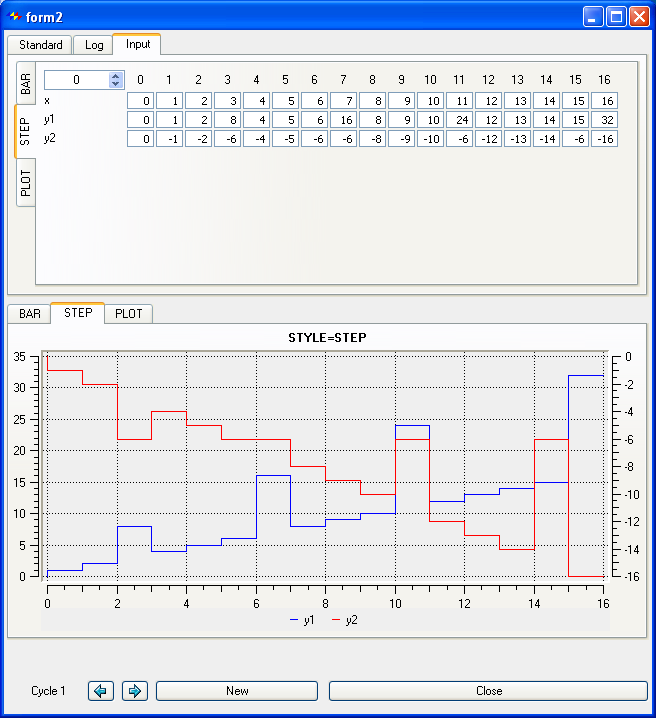
\includegraphics[width=280px]{grab_folder}
  \end{center}
  \caption{example of nested folders}
\end{figure}
